\documentclass{standalone}
\usepackage{tikz}
\usepackage{forest}
\usepackage{xcolor}
\def\es{edge from parent[solid]}
\def\ed{edge from parent[dashed]}
%\definecolor{fpgreen}{HTML}{A6D609}
\definecolor{fpgray}{HTML}{7B7B7C}
\definecolor{fpgost}{HTML}{FFFFFF}
\def\edm{edge from parent[dashed] [fpgost] node[auto=left] {\scriptsize ?} }
\begin{document}	
\centering
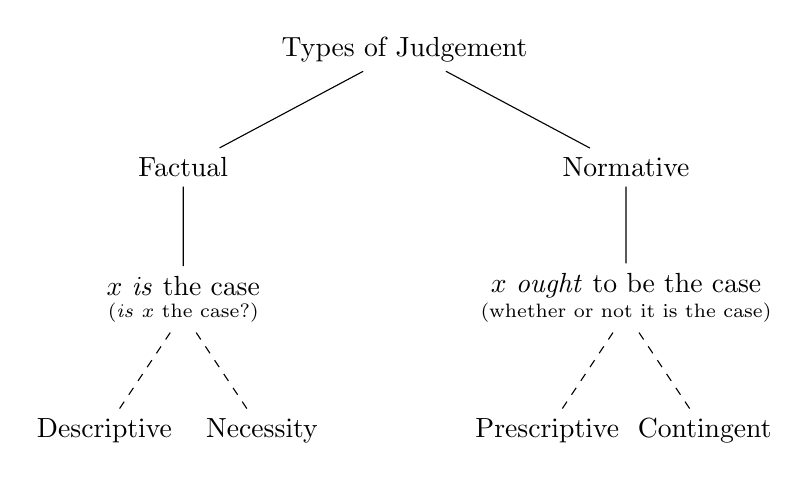
\begin{tikzpicture}[every node/.style={align=center},level 1/.style={sibling distance=8em},level 2/.style={sibling distance=20mm}, level 3/.style={sibling distance=40mm} level 4/.style={sibling distance=40mm}]

\node {Types of Judgement}
child { node {Factual}
    child { node (c) {\textit{$x$} \textit{is} the case} 
            node[below of= c, node distance=10pt] (a) {\scriptsize{(\textit{is} \textit{$x$} the case?)}}
            child {node {Descriptive} \ed}
            child {node {Necessity} \ed}}
}
% <- end fact
child {node [fpgost] {\scriptsize Moral} \edm } % <- end any, needs to be taken away.
% end moral
child { node {Normative}
    child{ node (y) {$x$ \textit{ought} to be the case}
           node [below of= y, node distance=10pt] (b) {\scriptsize{(whether or not it is the case)}}
        child {node {Prescriptive} \ed}
        child {node {Contingent} \ed}}
}; %<-end cognition

%% Extra lines
%%\draw[shorten >=0pt,dashed] (a)--(b); %node[midway,sloped, above] {compare};
\end{tikzpicture}
\end{document}